\documentclass[twoside]{book}

% Packages required by doxygen
\usepackage{fixltx2e}
\usepackage{calc}
\usepackage{doxygen}
\usepackage[export]{adjustbox} % also loads graphicx
\usepackage{graphicx}
\usepackage[utf8]{inputenc}
\usepackage{makeidx}
\usepackage{multicol}
\usepackage{multirow}
\PassOptionsToPackage{warn}{textcomp}
\usepackage{textcomp}
\usepackage[nointegrals]{wasysym}
\usepackage[table]{xcolor}

% Font selection
\usepackage[T1]{fontenc}
\usepackage[scaled=.90]{helvet}
\usepackage{courier}
\usepackage{amssymb}
\usepackage{sectsty}
\renewcommand{\familydefault}{\sfdefault}
\allsectionsfont{%
  \fontseries{bc}\selectfont%
  \color{darkgray}%
}
\renewcommand{\DoxyLabelFont}{%
  \fontseries{bc}\selectfont%
  \color{darkgray}%
}
\newcommand{\+}{\discretionary{\mbox{\scriptsize$\hookleftarrow$}}{}{}}

% Page & text layout
\usepackage{geometry}
\geometry{%
  a4paper,%
  top=2.5cm,%
  bottom=2.5cm,%
  left=2.5cm,%
  right=2.5cm%
}
\tolerance=750
\hfuzz=15pt
\hbadness=750
\setlength{\emergencystretch}{15pt}
\setlength{\parindent}{0cm}
\setlength{\parskip}{3ex plus 2ex minus 2ex}
\makeatletter
\renewcommand{\paragraph}{%
  \@startsection{paragraph}{4}{0ex}{-1.0ex}{1.0ex}{%
    \normalfont\normalsize\bfseries\SS@parafont%
  }%
}
\renewcommand{\subparagraph}{%
  \@startsection{subparagraph}{5}{0ex}{-1.0ex}{1.0ex}{%
    \normalfont\normalsize\bfseries\SS@subparafont%
  }%
}
\makeatother

% Headers & footers
\usepackage{fancyhdr}
\pagestyle{fancyplain}
\fancyhead[LE]{\fancyplain{}{\bfseries\thepage}}
\fancyhead[CE]{\fancyplain{}{}}
\fancyhead[RE]{\fancyplain{}{\bfseries\leftmark}}
\fancyhead[LO]{\fancyplain{}{\bfseries\rightmark}}
\fancyhead[CO]{\fancyplain{}{}}
\fancyhead[RO]{\fancyplain{}{\bfseries\thepage}}
\fancyfoot[LE]{\fancyplain{}{}}
\fancyfoot[CE]{\fancyplain{}{}}
\fancyfoot[RE]{\fancyplain{}{\bfseries\scriptsize Generated by Doxygen }}
\fancyfoot[LO]{\fancyplain{}{\bfseries\scriptsize Generated by Doxygen }}
\fancyfoot[CO]{\fancyplain{}{}}
\fancyfoot[RO]{\fancyplain{}{}}
\renewcommand{\footrulewidth}{0.4pt}
\renewcommand{\chaptermark}[1]{%
  \markboth{#1}{}%
}
\renewcommand{\sectionmark}[1]{%
  \markright{\thesection\ #1}%
}

% Indices & bibliography
\usepackage{natbib}
\usepackage[titles]{tocloft}
\setcounter{tocdepth}{3}
\setcounter{secnumdepth}{5}
\makeindex

% Custom commands
\newcommand{\clearemptydoublepage}{%
  \newpage{\pagestyle{empty}\cleardoublepage}%
}

\usepackage{caption}
\captionsetup{labelsep=space,justification=centering,font={bf},singlelinecheck=off,skip=4pt,position=top}

%===== C O N T E N T S =====

\begin{document}

% Titlepage & ToC
\pagenumbering{alph}
\begin{titlepage}
\vspace*{7cm}
\begin{center}%
{\Large My Project }\\
\vspace*{1cm}
{\large Generated by Doxygen 1.8.13}\\
\end{center}
\end{titlepage}
\clearemptydoublepage
\pagenumbering{roman}
\tableofcontents
\clearemptydoublepage
\pagenumbering{arabic}

%--- Begin generated contents ---
\chapter{Hierarchical Index}
\section{Class Hierarchy}
This inheritance list is sorted roughly, but not completely, alphabetically\+:\begin{DoxyCompactList}
\item \contentsline{section}{Interval}{\pageref{struct_interval}}{}
\item \contentsline{section}{Neuron}{\pageref{class_neuron}}{}
\begin{DoxyCompactList}
\item \contentsline{section}{Exhibitory}{\pageref{class_exhibitory}}{}
\item \contentsline{section}{Inhibitory}{\pageref{class_inhibitory}}{}
\end{DoxyCompactList}
\end{DoxyCompactList}

\chapter{Class Index}
\section{Class List}
Here are the classes, structs, unions and interfaces with brief descriptions\+:\begin{DoxyCompactList}
\item\contentsline{section}{\textbf{ Exhibitory} }{\pageref{class_exhibitory}}{}
\item\contentsline{section}{\textbf{ Inhibitory} }{\pageref{class_inhibitory}}{}
\item\contentsline{section}{\textbf{ Interval} \\*Structure for \doxyref{Interval}{p.}{struct_interval}. Since we enter an interval for our time limitations }{\pageref{struct_interval}}{}
\item\contentsline{section}{\textbf{ Neuron} }{\pageref{class_neuron}}{}
\end{DoxyCompactList}

\chapter{File Index}
\section{File List}
Here is a list of all files with brief descriptions\+:\begin{DoxyCompactList}
\item\contentsline{section}{\textbf{ constants.\+h} }{\pageref{constants_8h}}{}
\item\contentsline{section}{\textbf{ main.\+cpp} }{\pageref{main_8cpp}}{}
\item\contentsline{section}{\textbf{ neuron.\+cpp} }{\pageref{neuron_8cpp}}{}
\item\contentsline{section}{\textbf{ neuron.\+hpp} }{\pageref{neuron_8hpp}}{}
\item\contentsline{section}{\textbf{ unittest.\+cpp} }{\pageref{unittest_8cpp}}{}
\end{DoxyCompactList}

\chapter{Class Documentation}
\section{Exhibitory Class Reference}
\label{class_exhibitory}\index{Exhibitory@{Exhibitory}}


{\ttfamily \#include $<$neuron.\+hpp$>$}

Inheritance diagram for Exhibitory\+:\begin{figure}[H]
\begin{center}
\leavevmode
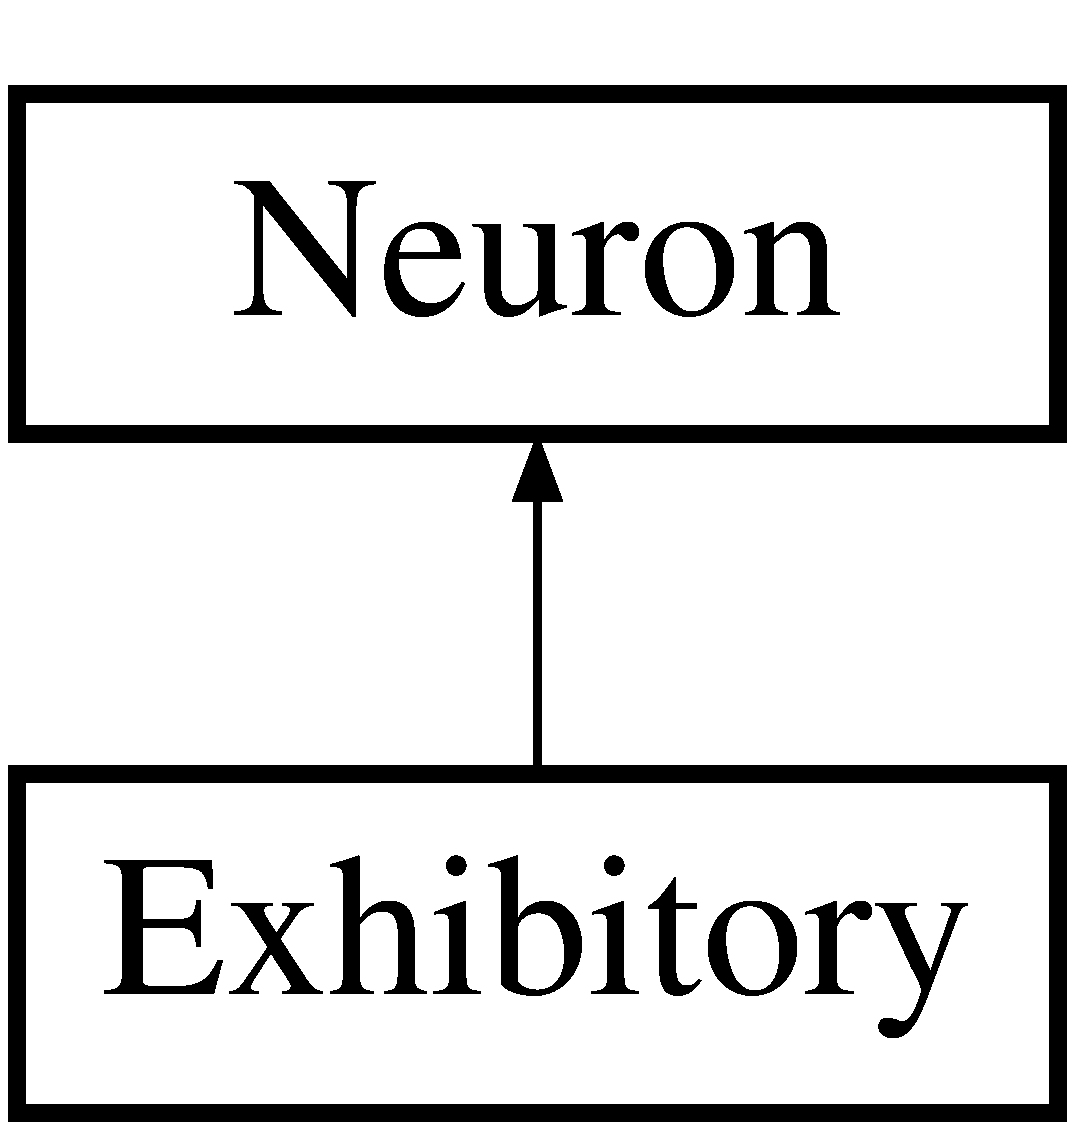
\includegraphics[height=2.000000cm]{class_exhibitory}
\end{center}
\end{figure}
\subsection*{Public Member Functions}
\begin{DoxyCompactItemize}
\item 
\textbf{ Exhibitory} ()
\begin{DoxyCompactList}\small\item\em Constructor. \end{DoxyCompactList}\end{DoxyCompactItemize}


\subsection{Detailed Description}
This class is for the exhibitory neurons, which have a different value for J. The only thing needed, is a constructor which initializes another value for J. 

\subsection{Constructor \& Destructor Documentation}
\mbox{\label{class_exhibitory_a067e5e9bc7881ac3671ec3320cacf7ef}} 
\index{Exhibitory@{Exhibitory}!Exhibitory@{Exhibitory}}
\index{Exhibitory@{Exhibitory}!Exhibitory@{Exhibitory}}
\subsubsection{Exhibitory()}
{\footnotesize\ttfamily Exhibitory\+::\+Exhibitory (\begin{DoxyParamCaption}{ }\end{DoxyParamCaption})\hspace{0.3cm}{\ttfamily [inline]}}



Constructor. 



The documentation for this class was generated from the following file\+:\begin{DoxyCompactItemize}
\item 
\textbf{ neuron.\+hpp}\end{DoxyCompactItemize}

\section{Inhibitory Class Reference}
\label{class_inhibitory}\index{Inhibitory@{Inhibitory}}


{\ttfamily \#include $<$neuron.\+hpp$>$}

Inheritance diagram for Inhibitory\+:\begin{figure}[H]
\begin{center}
\leavevmode
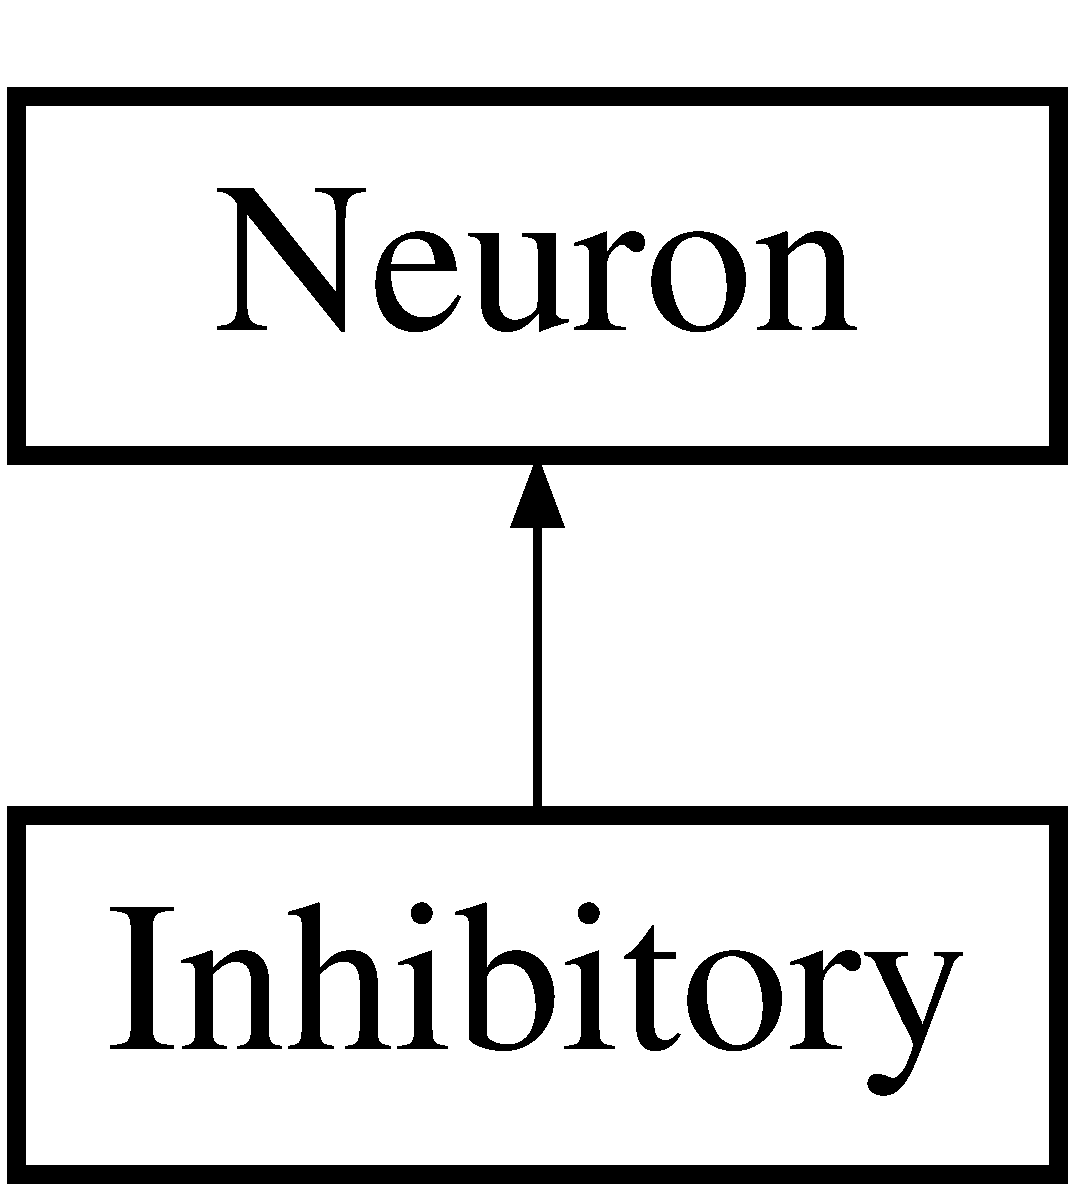
\includegraphics[height=2.000000cm]{class_inhibitory}
\end{center}
\end{figure}
\subsection*{Public Member Functions}
\begin{DoxyCompactItemize}
\item 
\textbf{ Inhibitory} ()
\begin{DoxyCompactList}\small\item\em Constructor. \end{DoxyCompactList}\end{DoxyCompactItemize}


\subsection{Detailed Description}
This class is for the inhibitory neurons, which have a different value for J. The only thing needed, is a constructor which initializes another value for J. 

\subsection{Constructor \& Destructor Documentation}
\mbox{\label{class_inhibitory_ae5bde3aa2eabeb2a6bb91deb6b9e6a1c}} 
\index{Inhibitory@{Inhibitory}!Inhibitory@{Inhibitory}}
\index{Inhibitory@{Inhibitory}!Inhibitory@{Inhibitory}}
\subsubsection{Inhibitory()}
{\footnotesize\ttfamily Inhibitory\+::\+Inhibitory (\begin{DoxyParamCaption}{ }\end{DoxyParamCaption})\hspace{0.3cm}{\ttfamily [inline]}}



Constructor. 



The documentation for this class was generated from the following file\+:\begin{DoxyCompactItemize}
\item 
\textbf{ neuron.\+hpp}\end{DoxyCompactItemize}

\section{Interval Struct Reference}
\label{struct_interval}\index{Interval@{Interval}}


Structure for \doxyref{Interval}{p.}{struct_interval}. Since we enter an interval for our time limitations.  


\subsection*{Public Attributes}
\begin{DoxyCompactItemize}
\item 
double \textbf{ start}
\item 
double \textbf{ end}
\end{DoxyCompactItemize}


\subsection{Detailed Description}
Structure for \doxyref{Interval}{p.}{struct_interval}. Since we enter an interval for our time limitations. 

\subsection{Member Data Documentation}
\mbox{\label{struct_interval_a3e157b77bf832e92c26fbe3283717d74}} 
\index{Interval@{Interval}!end@{end}}
\index{end@{end}!Interval@{Interval}}
\subsubsection{end}
{\footnotesize\ttfamily double Interval\+::end}

\mbox{\label{struct_interval_ae63ae31c07265309f48a39ce2472b692}} 
\index{Interval@{Interval}!start@{start}}
\index{start@{start}!Interval@{Interval}}
\subsubsection{start}
{\footnotesize\ttfamily double Interval\+::start}



The documentation for this struct was generated from the following file\+:\begin{DoxyCompactItemize}
\item 
\textbf{ main.\+cpp}\end{DoxyCompactItemize}

\section{Neuron Class Reference}
\label{class_neuron}\index{Neuron@{Neuron}}


{\ttfamily \#include $<$neuron.\+hpp$>$}

Inheritance diagram for Neuron\+:\begin{figure}[H]
\begin{center}
\leavevmode
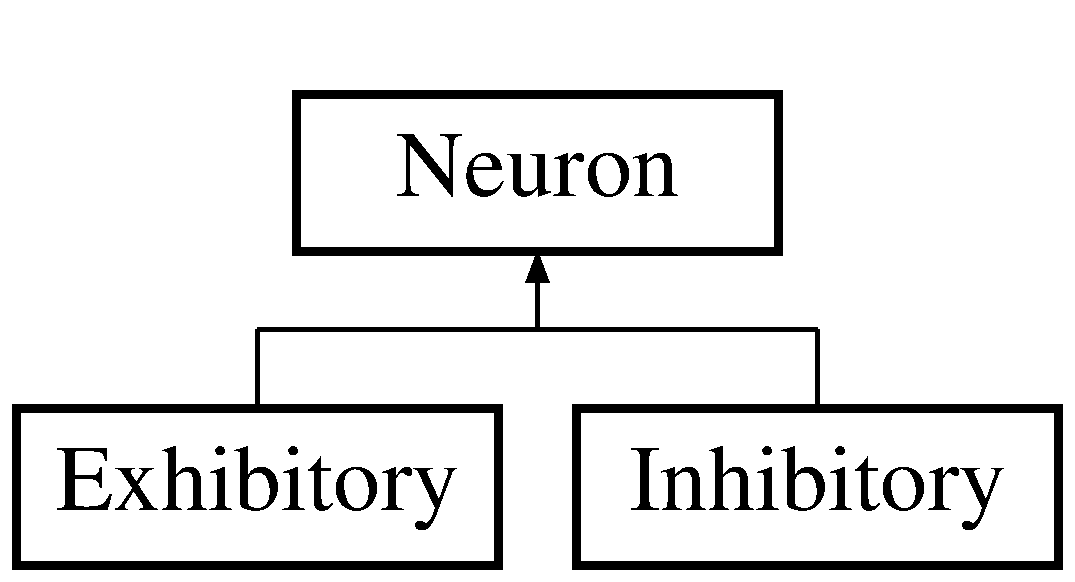
\includegraphics[height=2.000000cm]{class_neuron}
\end{center}
\end{figure}
\subsection*{Public Member Functions}
\begin{DoxyCompactItemize}
\item 
\textbf{ Neuron} ()
\begin{DoxyCompactList}\small\item\em This constructor is called if no arguments are passed. \end{DoxyCompactList}\item 
\textbf{ Neuron} (double Jvalue)
\begin{DoxyCompactList}\small\item\em This constructor is called if the value J has to be different. Ergo will be called by its subclasses. \end{DoxyCompactList}\item 
\textbf{ Neuron} (const \textbf{ Neuron} \&copy)=default
\begin{DoxyCompactList}\small\item\em Copy constructor. \end{DoxyCompactList}\item 
\textbf{ $\sim$\+Neuron} ()
\begin{DoxyCompactList}\small\item\em Destructor. \end{DoxyCompactList}\item 
void \textbf{ put\+In\+Vector} (double time)
\item 
bool \textbf{ update} (int time, double ext\+Curr)
\item 
bool \textbf{ spiked} ()
\item 
void \textbf{ add\+Connect} (\textbf{ Neuron} $\ast$other)
\item 
\textbf{ Neuron} $\ast$ \textbf{ get\+Connect\+Neuron} (int i)
\item 
bool \textbf{ receive} (int time)
\item 
bool \textbf{ clean\+Buffer} ()
\item 
bool \textbf{ destroy\+Connection} ()
\item 
double \textbf{ get\+Mem\+Pot} ()
\item 
double \textbf{ get\+Time\+Sp} ()
\item 
int \textbf{ get\+Clock} ()
\item 
int \textbf{ get\+Nbr\+Sp} ()
\item 
size\+\_\+t \textbf{ get\+Connec\+Size} ()
\item 
double \textbf{ get\+Spike\+Vect} (size\+\_\+t i)
\item 
size\+\_\+t \textbf{ get\+Spike\+Vect\+Size} ()
\end{DoxyCompactItemize}


\subsection{Constructor \& Destructor Documentation}
\mbox{\label{class_neuron_a823487d01615fadb8ac19a2768dd9d96}} 
\index{Neuron@{Neuron}!Neuron@{Neuron}}
\index{Neuron@{Neuron}!Neuron@{Neuron}}
\subsubsection{Neuron()\hspace{0.1cm}{\footnotesize\ttfamily [1/3]}}
{\footnotesize\ttfamily Neuron\+::\+Neuron (\begin{DoxyParamCaption}{ }\end{DoxyParamCaption})}



This constructor is called if no arguments are passed. 

$<$ For debugging purposes our first element of the connection vector is going to be a nullptr

$<$ Buffer of size (D/h+1), with all its entries to be zero \mbox{\label{class_neuron_a08113313e9b6c871c8ce2e813d7f14d5}} 
\index{Neuron@{Neuron}!Neuron@{Neuron}}
\index{Neuron@{Neuron}!Neuron@{Neuron}}
\subsubsection{Neuron()\hspace{0.1cm}{\footnotesize\ttfamily [2/3]}}
{\footnotesize\ttfamily Neuron\+::\+Neuron (\begin{DoxyParamCaption}\item[{double}]{Jvalue }\end{DoxyParamCaption})}



This constructor is called if the value J has to be different. Ergo will be called by its subclasses. 

$<$ For debugging purposes our first element of the connection vector is going to be a nullptr

$<$ Buffer of size (D/h+1), with all its entries to be zero \mbox{\label{class_neuron_a12d7fc474ce96416f151099880596cbb}} 
\index{Neuron@{Neuron}!Neuron@{Neuron}}
\index{Neuron@{Neuron}!Neuron@{Neuron}}
\subsubsection{Neuron()\hspace{0.1cm}{\footnotesize\ttfamily [3/3]}}
{\footnotesize\ttfamily Neuron\+::\+Neuron (\begin{DoxyParamCaption}\item[{const \textbf{ Neuron} \&}]{copy }\end{DoxyParamCaption})\hspace{0.3cm}{\ttfamily [default]}}



Copy constructor. 

\mbox{\label{class_neuron_a94a250ce7e167760e593979b899745b1}} 
\index{Neuron@{Neuron}!````~Neuron@{$\sim$\+Neuron}}
\index{````~Neuron@{$\sim$\+Neuron}!Neuron@{Neuron}}
\subsubsection{$\sim$\+Neuron()}
{\footnotesize\ttfamily Neuron\+::$\sim$\+Neuron (\begin{DoxyParamCaption}{ }\end{DoxyParamCaption})\hspace{0.3cm}{\ttfamily [inline]}}



Destructor. 



\subsection{Member Function Documentation}
\mbox{\label{class_neuron_a337162e9c43f40516784b649f07ee0f9}} 
\index{Neuron@{Neuron}!add\+Connect@{add\+Connect}}
\index{add\+Connect@{add\+Connect}!Neuron@{Neuron}}
\subsubsection{add\+Connect()}
{\footnotesize\ttfamily void Neuron\+::add\+Connect (\begin{DoxyParamCaption}\item[{\textbf{ Neuron} $\ast$}]{other }\end{DoxyParamCaption})}

This function is responsible to connect neurons together, it pushes the new connected neuron in the existing connection vector. 
\begin{DoxyParams}{Parameters}
{\em neuron} & that it is gonna be connected to \\
\hline
\end{DoxyParams}
\mbox{\label{class_neuron_a931fddbafb3c4a5220dfe2d40e0fc249}} 
\index{Neuron@{Neuron}!clean\+Buffer@{clean\+Buffer}}
\index{clean\+Buffer@{clean\+Buffer}!Neuron@{Neuron}}
\subsubsection{clean\+Buffer()}
{\footnotesize\ttfamily bool Neuron\+::clean\+Buffer (\begin{DoxyParamCaption}{ }\end{DoxyParamCaption})}

This function has been created for debugging porpuses only. It makes the code also more readable. \begin{DoxyReturn}{Returns}
true if the buffer elements have been set to 0 
\end{DoxyReturn}
\mbox{\label{class_neuron_a77b6781a4864753504cb6c26f00c61a2}} 
\index{Neuron@{Neuron}!destroy\+Connection@{destroy\+Connection}}
\index{destroy\+Connection@{destroy\+Connection}!Neuron@{Neuron}}
\subsubsection{destroy\+Connection()}
{\footnotesize\ttfamily bool Neuron\+::destroy\+Connection (\begin{DoxyParamCaption}{ }\end{DoxyParamCaption})}

This function will be called in the very end to free and delete the pointers of the connection vector. \begin{DoxyReturn}{Returns}
true if the pointers have been freed 
\end{DoxyReturn}
$<$ if connection vector is not empty assert \mbox{\label{class_neuron_a0c6f3326a19ca4623f7a53b4b82e69ce}} 
\index{Neuron@{Neuron}!get\+Clock@{get\+Clock}}
\index{get\+Clock@{get\+Clock}!Neuron@{Neuron}}
\subsubsection{get\+Clock()}
{\footnotesize\ttfamily int Neuron\+::get\+Clock (\begin{DoxyParamCaption}{ }\end{DoxyParamCaption})\hspace{0.3cm}{\ttfamily [inline]}}

\mbox{\label{class_neuron_a68bd47e91a15162f7ce767c5350260f2}} 
\index{Neuron@{Neuron}!get\+Connec\+Size@{get\+Connec\+Size}}
\index{get\+Connec\+Size@{get\+Connec\+Size}!Neuron@{Neuron}}
\subsubsection{get\+Connec\+Size()}
{\footnotesize\ttfamily size\+\_\+t Neuron\+::get\+Connec\+Size (\begin{DoxyParamCaption}{ }\end{DoxyParamCaption})\hspace{0.3cm}{\ttfamily [inline]}}

\mbox{\label{class_neuron_a94672ed8219d66ee2fa6c73bec1c775b}} 
\index{Neuron@{Neuron}!get\+Connect\+Neuron@{get\+Connect\+Neuron}}
\index{get\+Connect\+Neuron@{get\+Connect\+Neuron}!Neuron@{Neuron}}
\subsubsection{get\+Connect\+Neuron()}
{\footnotesize\ttfamily \textbf{ Neuron} $\ast$ Neuron\+::get\+Connect\+Neuron (\begin{DoxyParamCaption}\item[{int}]{i }\end{DoxyParamCaption})}

This function is responsible to show to which neuron it is connected to. It is mainly done to make the private vector connection to be accessible to be read. 
\begin{DoxyParams}{Parameters}
{\em i} & is the place in the vector that we wannt to look at \\
\hline
\end{DoxyParams}
\begin{DoxyReturn}{Returns}
neuron at that certain place of the connection vector 
\end{DoxyReturn}
$<$ A\+T\+T\+E\+N\+T\+I\+ON\+: connection vector has a nullptr as first element \mbox{\label{class_neuron_a8662cd2c161850aa1141ba0d9247e476}} 
\index{Neuron@{Neuron}!get\+Mem\+Pot@{get\+Mem\+Pot}}
\index{get\+Mem\+Pot@{get\+Mem\+Pot}!Neuron@{Neuron}}
\subsubsection{get\+Mem\+Pot()}
{\footnotesize\ttfamily double Neuron\+::get\+Mem\+Pot (\begin{DoxyParamCaption}{ }\end{DoxyParamCaption})\hspace{0.3cm}{\ttfamily [inline]}}

\mbox{\label{class_neuron_a2656be288ae861cf0b2b815adcfef622}} 
\index{Neuron@{Neuron}!get\+Nbr\+Sp@{get\+Nbr\+Sp}}
\index{get\+Nbr\+Sp@{get\+Nbr\+Sp}!Neuron@{Neuron}}
\subsubsection{get\+Nbr\+Sp()}
{\footnotesize\ttfamily int Neuron\+::get\+Nbr\+Sp (\begin{DoxyParamCaption}{ }\end{DoxyParamCaption})\hspace{0.3cm}{\ttfamily [inline]}}

\mbox{\label{class_neuron_a30899cfd423bf99b7faf944e77f6bc97}} 
\index{Neuron@{Neuron}!get\+Spike\+Vect@{get\+Spike\+Vect}}
\index{get\+Spike\+Vect@{get\+Spike\+Vect}!Neuron@{Neuron}}
\subsubsection{get\+Spike\+Vect()}
{\footnotesize\ttfamily double Neuron\+::get\+Spike\+Vect (\begin{DoxyParamCaption}\item[{size\+\_\+t}]{i }\end{DoxyParamCaption})\hspace{0.3cm}{\ttfamily [inline]}}

\mbox{\label{class_neuron_ad9141cb0791f75a92f0b9d1543346193}} 
\index{Neuron@{Neuron}!get\+Spike\+Vect\+Size@{get\+Spike\+Vect\+Size}}
\index{get\+Spike\+Vect\+Size@{get\+Spike\+Vect\+Size}!Neuron@{Neuron}}
\subsubsection{get\+Spike\+Vect\+Size()}
{\footnotesize\ttfamily size\+\_\+t Neuron\+::get\+Spike\+Vect\+Size (\begin{DoxyParamCaption}{ }\end{DoxyParamCaption})\hspace{0.3cm}{\ttfamily [inline]}}

\mbox{\label{class_neuron_af4f57ac98e4be891d6e1b04d131a28dd}} 
\index{Neuron@{Neuron}!get\+Time\+Sp@{get\+Time\+Sp}}
\index{get\+Time\+Sp@{get\+Time\+Sp}!Neuron@{Neuron}}
\subsubsection{get\+Time\+Sp()}
{\footnotesize\ttfamily double Neuron\+::get\+Time\+Sp (\begin{DoxyParamCaption}{ }\end{DoxyParamCaption})\hspace{0.3cm}{\ttfamily [inline]}}

\mbox{\label{class_neuron_a00617ab481fd653493257c84b4e07dda}} 
\index{Neuron@{Neuron}!put\+In\+Vector@{put\+In\+Vector}}
\index{put\+In\+Vector@{put\+In\+Vector}!Neuron@{Neuron}}
\subsubsection{put\+In\+Vector()}
{\footnotesize\ttfamily void Neuron\+::put\+In\+Vector (\begin{DoxyParamCaption}\item[{double}]{time }\end{DoxyParamCaption})}

This function is responsible to push back given times into the spike\+Vect vector, which we later on need to write into the spike.\+txt file. 
\begin{DoxyParams}{Parameters}
{\em time} & the spike occured and has to be saved. \\
\hline
\end{DoxyParams}
\mbox{\label{class_neuron_a6cc00373ace5406d18a4673a82ba0e09}} 
\index{Neuron@{Neuron}!receive@{receive}}
\index{receive@{receive}!Neuron@{Neuron}}
\subsubsection{receive()}
{\footnotesize\ttfamily bool Neuron\+::receive (\begin{DoxyParamCaption}\item[{int}]{time }\end{DoxyParamCaption})}

This function is responsible to make a neuron receive all the spikes it gets from its connected neurons and to reset the buffer if necessary. 
\begin{DoxyParams}{Parameters}
{\em time} & is the global time we need to check where we are at in the buffer \\
\hline
\end{DoxyParams}
\begin{DoxyReturn}{Returns}
true if neuron received spike -\/$>$ debug purposes 
\end{DoxyReturn}
If time is smaller then buffer\+Size we can store +1 at time

$<$ delay D taken in account when function is called

$<$ assert if time is negative -\/$>$ at least 15! bc delay has been added

Store +1 in buffer Modulo will not work for timesteps that are smaller then buffer\+Size (only 15 bc of delay)

If time is overexceeding buffer\+Size, we need to start from the beginning again to store it at correct place

$<$ Set buffer all to 0 because we overexceeded it and we \char`\"{}start\char`\"{} from new with the vector

$<$ assert if buffer has not been cleaned

$<$ assert if store\+Time is bigger then the buffersize

time\+Step is now garantueed smaller then buffersize, so we store +1 \mbox{\label{class_neuron_a95efbf8af058ce38307abc4c229ed046}} 
\index{Neuron@{Neuron}!spiked@{spiked}}
\index{spiked@{spiked}!Neuron@{Neuron}}
\subsubsection{spiked()}
{\footnotesize\ttfamily bool Neuron\+::spiked (\begin{DoxyParamCaption}{ }\end{DoxyParamCaption})}

This function is responsible to tell if the neuron spikes.

\begin{DoxyReturn}{Returns}
true if the neuron spikes false if the neuron doesn\textquotesingle{}t spike 
\end{DoxyReturn}
\mbox{\label{class_neuron_a0e559ebeedcccc021e976d38d3fca3fa}} 
\index{Neuron@{Neuron}!update@{update}}
\index{update@{update}!Neuron@{Neuron}}
\subsubsection{update()}
{\footnotesize\ttfamily bool Neuron\+::update (\begin{DoxyParamCaption}\item[{int}]{time,  }\item[{double}]{ext\+Curr }\end{DoxyParamCaption})}

This function is responsible to update the neuron, meaning it resets the membrane potential, taking account how many spikes it receives and what randomly generated background noise it gets. 
\begin{DoxyParams}{Parameters}
{\em time} & is the global time, to see where we are at \\
\hline
{\em ext\+Curr} & is the external current which has in ealier steps been entered in the main and now is set to 0 \\
\hline
\end{DoxyParams}
\begin{DoxyReturn}{Returns}
true if neuron spiked 
\end{DoxyReturn}
Since buffer has size D/h+1 the time is going to exceed it fast. Therefore we interate through the buffervector and start again everytime when we exceed it, we take the modulo of the time\+Step and the buffersize to be sure where to access the buffer at.

Count the spikes received at time

$<$ first time step is at the zero element of vector and we start with time 0

The whole clocksystem is in steps, therefore the refractorytime has to be used in steps as well

$<$ Refractorytime is for sure never gonna be 0; so neither is the steps

The neuron is insensitiv for a refacttime If my spike\+Vect is not empty, then check when neuron has had last spike

$<$ If last spike as occured less then refracttime ago

Generating background noise of the brain by possion distribution

$<$ Pois() gives me back an int as default

$<$ change type

$<$ assert -\/$>$ background noise can\textquotesingle{}t be negativ (Pois() is never negative)

Calculate membrane potential

Set it as new potential

Check if neuron spiked

$<$ Increase the nbr of spikes the neuron itself has

$<$ Store the time in the spike vector and set spike time 

The documentation for this class was generated from the following files\+:\begin{DoxyCompactItemize}
\item 
\textbf{ neuron.\+hpp}\item 
\textbf{ neuron.\+cpp}\end{DoxyCompactItemize}

\chapter{File Documentation}
\section{constants.\+h File Reference}
\label{constants_8h}\index{constants.\+h@{constants.\+h}}
\subsection*{Variables}
\begin{DoxyCompactItemize}
\item 
const double \textbf{ tau} = 20
\begin{DoxyCompactList}\small\item\em ms constant \end{DoxyCompactList}\item 
const double \textbf{ h} = 0.\+1
\begin{DoxyCompactList}\small\item\em ms constant \end{DoxyCompactList}\item 
const double \textbf{ R} = 20
\begin{DoxyCompactList}\small\item\em constant \end{DoxyCompactList}\item 
const double \textbf{ treshold} = 20
\begin{DoxyCompactList}\small\item\em mV potential when it spikes \end{DoxyCompactList}\item 
const double \textbf{ refactime} = 2
\begin{DoxyCompactList}\small\item\em ms time it takes to be able to take another spike \end{DoxyCompactList}\item 
const double \textbf{ J} = 0.\+1
\begin{DoxyCompactList}\small\item\em mV potential given by background \end{DoxyCompactList}\item 
const int \textbf{ g} = 5
\begin{DoxyCompactList}\small\item\em ratio Ji/\+Je -\/$>$ can be changed for different graphs \end{DoxyCompactList}\item 
const double \textbf{ D} = 1.\+5
\begin{DoxyCompactList}\small\item\em ms delay because of distance of neurons \end{DoxyCompactList}\item 
const int \textbf{ buffer\+Size} = static\+\_\+cast$<$int$>$(\textbf{ D}/\textbf{ h}) + 1
\begin{DoxyCompactList}\small\item\em size of buffer vector -\/$>$ instead of calculating it each time \end{DoxyCompactList}\item 
const double \textbf{ Je} = 0.\+1
\begin{DoxyCompactList}\small\item\em mV potential given by a exhibitory neuron \end{DoxyCompactList}\item 
const double \textbf{ Ji} = -\/\textbf{ Je} $\ast$ \textbf{ g}
\begin{DoxyCompactList}\small\item\em mv potential given by a inhibitory neuron \end{DoxyCompactList}\item 
const int \textbf{ Ne} = 10000
\begin{DoxyCompactList}\small\item\em amount of exhib neurons \end{DoxyCompactList}\item 
const int \textbf{ Ni} = 2500
\begin{DoxyCompactList}\small\item\em amount of inhib neurons \end{DoxyCompactList}\item 
const int \textbf{ Ce} = \textbf{ Ne}/10
\begin{DoxyCompactList}\small\item\em amount of connection exhibitory \end{DoxyCompactList}\item 
const int \textbf{ Ci} = \textbf{ Ni}/10
\begin{DoxyCompactList}\small\item\em amount of connection inhibitory \end{DoxyCompactList}\item 
const double \textbf{ frequency\+Th} = \textbf{ treshold}/(\textbf{ Ce}$\ast$\textbf{ Je}$\ast$\textbf{ tau})
\begin{DoxyCompactList}\small\item\em Variables for distributions. \end{DoxyCompactList}\item 
const double \textbf{ frequency\+Ext} = 2 $\ast$ \textbf{ frequency\+Th}
\item 
const double \textbf{ lambda} = \textbf{ frequency\+Ext} $\ast$ \textbf{ Ne} $\ast$ \textbf{ h} $\ast$ \textbf{ Je}
\begin{DoxyCompactList}\small\item\em constant to be used in possiondistribution \end{DoxyCompactList}\end{DoxyCompactItemize}


\subsection{Variable Documentation}
\mbox{\label{constants_8h_a4cb7aa26412b9517e92b492fa0386879}} 
\index{constants.\+h@{constants.\+h}!buffer\+Size@{buffer\+Size}}
\index{buffer\+Size@{buffer\+Size}!constants.\+h@{constants.\+h}}
\subsubsection{buffer\+Size}
{\footnotesize\ttfamily const int buffer\+Size = static\+\_\+cast$<$int$>$(\textbf{ D}/\textbf{ h}) + 1}



size of buffer vector -\/$>$ instead of calculating it each time 

specific values for in-\//exhibitory neurons \mbox{\label{constants_8h_a4a9fd51283b56aa467c2c1897f1f91f7}} 
\index{constants.\+h@{constants.\+h}!Ce@{Ce}}
\index{Ce@{Ce}!constants.\+h@{constants.\+h}}
\subsubsection{Ce}
{\footnotesize\ttfamily const int Ce = \textbf{ Ne}/10}



amount of connection exhibitory 

\mbox{\label{constants_8h_ad5c0cafea18f89372a01f215f23976bb}} 
\index{constants.\+h@{constants.\+h}!Ci@{Ci}}
\index{Ci@{Ci}!constants.\+h@{constants.\+h}}
\subsubsection{Ci}
{\footnotesize\ttfamily const int Ci = \textbf{ Ni}/10}



amount of connection inhibitory 

\mbox{\label{constants_8h_a412464ee5e4d4e873c365d926d1970bb}} 
\index{constants.\+h@{constants.\+h}!D@{D}}
\index{D@{D}!constants.\+h@{constants.\+h}}
\subsubsection{D}
{\footnotesize\ttfamily const double D = 1.\+5}



ms delay because of distance of neurons 

\mbox{\label{constants_8h_afb508c9e901b233efc4bfaa68d629570}} 
\index{constants.\+h@{constants.\+h}!frequency\+Ext@{frequency\+Ext}}
\index{frequency\+Ext@{frequency\+Ext}!constants.\+h@{constants.\+h}}
\subsubsection{frequency\+Ext}
{\footnotesize\ttfamily const double frequency\+Ext = 2 $\ast$ \textbf{ frequency\+Th}}

\mbox{\label{constants_8h_a35bcf347fb4545809fe41b549784498a}} 
\index{constants.\+h@{constants.\+h}!frequency\+Th@{frequency\+Th}}
\index{frequency\+Th@{frequency\+Th}!constants.\+h@{constants.\+h}}
\subsubsection{frequency\+Th}
{\footnotesize\ttfamily const double frequency\+Th = \textbf{ treshold}/(\textbf{ Ce}$\ast$\textbf{ Je}$\ast$\textbf{ tau})}



Variables for distributions. 

\mbox{\label{constants_8h_aece2eeedca2f58e31a680503a9b7e972}} 
\index{constants.\+h@{constants.\+h}!g@{g}}
\index{g@{g}!constants.\+h@{constants.\+h}}
\subsubsection{g}
{\footnotesize\ttfamily const int g = 5}



ratio Ji/\+Je -\/$>$ can be changed for different graphs 

\mbox{\label{constants_8h_aa6e8e201edf24007dc075bfef6e8210c}} 
\index{constants.\+h@{constants.\+h}!h@{h}}
\index{h@{h}!constants.\+h@{constants.\+h}}
\subsubsection{h}
{\footnotesize\ttfamily const double h = 0.\+1}



ms constant 

\mbox{\label{constants_8h_abb4f6430d98825c1e2344074ee09c57a}} 
\index{constants.\+h@{constants.\+h}!J@{J}}
\index{J@{J}!constants.\+h@{constants.\+h}}
\subsubsection{J}
{\footnotesize\ttfamily const double J = 0.\+1}



mV potential given by background 

\mbox{\label{constants_8h_a39898975b4c6d6a29e121e7e4b350a2c}} 
\index{constants.\+h@{constants.\+h}!Je@{Je}}
\index{Je@{Je}!constants.\+h@{constants.\+h}}
\subsubsection{Je}
{\footnotesize\ttfamily const double Je = 0.\+1}



mV potential given by a exhibitory neuron 

\mbox{\label{constants_8h_ac96467d7ddc139a268b00c766205fd04}} 
\index{constants.\+h@{constants.\+h}!Ji@{Ji}}
\index{Ji@{Ji}!constants.\+h@{constants.\+h}}
\subsubsection{Ji}
{\footnotesize\ttfamily const double Ji = -\/\textbf{ Je} $\ast$ \textbf{ g}}



mv potential given by a inhibitory neuron 

\mbox{\label{constants_8h_a01c828218289eff2af40b9cdf043393f}} 
\index{constants.\+h@{constants.\+h}!lambda@{lambda}}
\index{lambda@{lambda}!constants.\+h@{constants.\+h}}
\subsubsection{lambda}
{\footnotesize\ttfamily const double lambda = \textbf{ frequency\+Ext} $\ast$ \textbf{ Ne} $\ast$ \textbf{ h} $\ast$ \textbf{ Je}}



constant to be used in possiondistribution 

\mbox{\label{constants_8h_a78f078e19c99a6fc51a8bc2adb8acfa0}} 
\index{constants.\+h@{constants.\+h}!Ne@{Ne}}
\index{Ne@{Ne}!constants.\+h@{constants.\+h}}
\subsubsection{Ne}
{\footnotesize\ttfamily const int Ne = 10000}



amount of exhib neurons 

\mbox{\label{constants_8h_a7f259aefd534417d68d4587e7eaacc55}} 
\index{constants.\+h@{constants.\+h}!Ni@{Ni}}
\index{Ni@{Ni}!constants.\+h@{constants.\+h}}
\subsubsection{Ni}
{\footnotesize\ttfamily const int Ni = 2500}



amount of inhib neurons 

\mbox{\label{constants_8h_a0877420f3d7b1f47b871d2ccb47168d8}} 
\index{constants.\+h@{constants.\+h}!R@{R}}
\index{R@{R}!constants.\+h@{constants.\+h}}
\subsubsection{R}
{\footnotesize\ttfamily const double R = 20}



constant 

\mbox{\label{constants_8h_af4833bd02aabd3f9bd897677d3a4acb1}} 
\index{constants.\+h@{constants.\+h}!refactime@{refactime}}
\index{refactime@{refactime}!constants.\+h@{constants.\+h}}
\subsubsection{refactime}
{\footnotesize\ttfamily const double refactime = 2}



ms time it takes to be able to take another spike 

\mbox{\label{constants_8h_a9a42c4d90eb9808c60bb3f1be6a0c1a7}} 
\index{constants.\+h@{constants.\+h}!tau@{tau}}
\index{tau@{tau}!constants.\+h@{constants.\+h}}
\subsubsection{tau}
{\footnotesize\ttfamily const double tau = 20}



ms constant 

$<$ constants.\+h SV Project

Created by Samara Frey on 02.\+10.\+17. Copyright © 2017 Samara Frey. All rights reserved. This file contains all the constant we use for the equations All the time measurments will be in ms. All the potentials are in mV. \mbox{\label{constants_8h_a82a0ca3ab70a0a31c932651ac335723a}} 
\index{constants.\+h@{constants.\+h}!treshold@{treshold}}
\index{treshold@{treshold}!constants.\+h@{constants.\+h}}
\subsubsection{treshold}
{\footnotesize\ttfamily const double treshold = 20}



mV potential when it spikes 


\section{main.\+cpp File Reference}
\label{main_8cpp}\index{main.\+cpp@{main.\+cpp}}
{\ttfamily \#include \char`\"{}neuron.\+hpp\char`\"{}}\newline
{\ttfamily \#include \char`\"{}constants.\+h\char`\"{}}\newline
{\ttfamily \#include $<$cmath$>$}\newline
{\ttfamily \#include $<$cassert$>$}\newline
{\ttfamily \#include $<$iostream$>$}\newline
{\ttfamily \#include $<$random$>$}\newline
{\ttfamily \#include $<$fstream$>$}\newline
\subsection*{Classes}
\begin{DoxyCompactItemize}
\item 
struct \textbf{ Interval}
\begin{DoxyCompactList}\small\item\em Structure for \doxyref{Interval}{p.}{struct_interval}. Since we enter an interval for our time limitations. \end{DoxyCompactList}\end{DoxyCompactItemize}
\subsection*{Functions}
\begin{DoxyCompactItemize}
\item 
void \textbf{ check\+Value} (double value)
\begin{DoxyCompactList}\small\item\em $<$ to check value \end{DoxyCompactList}\item 
\textbf{ Interval} \textbf{ set\+Interval} ()
\item 
void \textbf{ explain\+Values} ()
\item 
vector$<$ int $>$ \textbf{ get\+Random} (int nbr\+Choose, int i)
\item 
int \textbf{ main} ()
\end{DoxyCompactItemize}


\subsection{Function Documentation}
\mbox{\label{main_8cpp_af86d5b91822a38a917e8bf420581425e}} 
\index{main.\+cpp@{main.\+cpp}!check\+Value@{check\+Value}}
\index{check\+Value@{check\+Value}!main.\+cpp@{main.\+cpp}}
\subsubsection{check\+Value()}
{\footnotesize\ttfamily void check\+Value (\begin{DoxyParamCaption}\item[{double}]{value }\end{DoxyParamCaption})}



$<$ to check value 

Checking values. If vaules are not as expected, cout a warning message before ending programm. 
\begin{DoxyParams}{Parameters}
{\em value} & the value that has to be checked. \\
\hline
\end{DoxyParams}
\mbox{\label{main_8cpp_afd8975ff2a6235c3d1f28f95223c4d46}} 
\index{main.\+cpp@{main.\+cpp}!explain\+Values@{explain\+Values}}
\index{explain\+Values@{explain\+Values}!main.\+cpp@{main.\+cpp}}
\subsubsection{explain\+Values()}
{\footnotesize\ttfamily void explain\+Values (\begin{DoxyParamCaption}{ }\end{DoxyParamCaption})}

This function is responsible to tell the User whith which values he is dealing with. If he is not happy with them he can directly stop the programm and change the values in the constant file accordingly. \mbox{\label{main_8cpp_a0d9e56d959df537267c02e52c5badcb1}} 
\index{main.\+cpp@{main.\+cpp}!get\+Random@{get\+Random}}
\index{get\+Random@{get\+Random}!main.\+cpp@{main.\+cpp}}
\subsubsection{get\+Random()}
{\footnotesize\ttfamily vector$<$ int $>$ get\+Random (\begin{DoxyParamCaption}\item[{int}]{nbr\+Choose,  }\item[{int}]{i }\end{DoxyParamCaption})}

This function is responsible to create x random numbers and store then in a vector. We always need to create nbr\+Choose/10. Which would be Ce or Ci depending on which neuron I want to connect. A\+T\+T\+E\+N\+T\+I\+ON\+: the random number can\textquotesingle{}t be i, because the neuron can technically not be connected to itself. 
\begin{DoxyParams}{Parameters}
{\em nbr\+Choose} & is the \char`\"{}pot\char`\"{} of numbers where we can choose from \\
\hline
{\em i} & is the only number we should not generate \\
\hline
\end{DoxyParams}
$<$ Size is 10th of nbrs to choose from (10\textquotesingle{}000 -\/$>$ 1\textquotesingle{}000; 2\textquotesingle{}500 -\/$>$ 250)

$<$ Exclude the option to be connected with itself \mbox{\label{main_8cpp_ae66f6b31b5ad750f1fe042a706a4e3d4}} 
\index{main.\+cpp@{main.\+cpp}!main@{main}}
\index{main@{main}!main.\+cpp@{main.\+cpp}}
\subsubsection{main()}
{\footnotesize\ttfamily int main (\begin{DoxyParamCaption}{ }\end{DoxyParamCaption})}

Make sure the User knows with which values he deals

$<$ vectors with all the neurons ex and in

Creating a set of Neurons

Simplicitywise first store all ex (Ne) and then all in (Ni) in the all\+Neuron vector. Start with pushing back Ne exhibitory neurons, then Ni inhibitory neurons.

Create random connections inbetween Neurons

Connect each neuron to Ce exhib neurons. Start with connection exhib neurons (they are the first in the all\+Neuron vector, then connect inhib neurons.

$<$ generate vector (size Ce) with random nbrs from 0 to Ne-\/1 for exhib connections

$<$ having exhibitory neurons from 0th element on

$<$ start having inhibitory neurons from 10\textquotesingle{}000th element on

Connect each neuron to Ci inhib neurons. Start with connection exhib neurons (they are the first in the all\+Neuron vector, then connect inhib neurons.

Attention\+: inhibitory neurons start from the Ne\textquotesingle{}s value on and we want to go till the end which is at Ne+\+Ni (vector starts with 0)

$<$ generate vector (size Ce) with random nbrs from 0 to Ne-\/1 for exhib connections

$<$ having exhibitory neurons from 0th element on

$<$ start having inhibitory neurons from 10\textquotesingle{}000th element on

Start of global clock

Get the time interval, external current is 0 Attention\+: Time interval entered is in ms, we work with 0.\+1ms time steps

Programm works with time steps, convert time

Open a new file

Check that file are open

Check that opening of file didn\textquotesingle{}t fail

Entering simulation which runs for the entered time \doxyref{Interval}{p.}{struct_interval}

This simulation iterates for the time we entered before. It works with 0.\+1ms time steps and updates each neuron of the all\+Neuron vector for each time step. It is responsible to coordinate the receiving and giving of time spikes to connected neurons. In addition to this, we store the new generated membrane potential in a seperate file which has been opened before.

Check if neuron spiked -\/$>$ if yes tell its connected neurons

$<$ If spiked tell to buffers of connected neurons p starts from 1 because nullptr is first element

$<$ Delay added

Store and delete data generated

Here we store the data of the spikes in a seperate file which has been opened before. We need this for being able to recreate the histogramm and other graphs. In the iteration we also free and delete the pointers of the connection vector of each neuron. The destructor of the neuron will be called automatically at the end of the programm -\/$>$ no need to call it manually.

ms

$<$ store the spike times in file

Close the file that we have written into \mbox{\label{main_8cpp_a3733080ed023d8e513d379e329a58c85}} 
\index{main.\+cpp@{main.\+cpp}!set\+Interval@{set\+Interval}}
\index{set\+Interval@{set\+Interval}!main.\+cpp@{main.\+cpp}}
\subsubsection{set\+Interval()}
{\footnotesize\ttfamily \textbf{ Interval} set\+Interval (\begin{DoxyParamCaption}{ }\end{DoxyParamCaption})}

Setting the \doxyref{Interval}{p.}{struct_interval} bonds. \doxyref{Interval}{p.}{struct_interval} is a structure that has been created. Entered values will always be checked. \begin{DoxyReturn}{Returns}
interval which has been entered. 
\end{DoxyReturn}

\section{neuron.\+cpp File Reference}
\label{neuron_8cpp}\index{neuron.\+cpp@{neuron.\+cpp}}
{\ttfamily \#include \char`\"{}neuron.\+hpp\char`\"{}}\newline
{\ttfamily \#include \char`\"{}constants.\+h\char`\"{}}\newline
{\ttfamily \#include $<$cassert$>$}\newline
{\ttfamily \#include $<$iostream$>$}\newline
{\ttfamily \#include $<$cmath$>$}\newline
{\ttfamily \#include $<$vector$>$}\newline
{\ttfamily \#include $<$random$>$}\newline

\section{neuron.\+hpp File Reference}
\label{neuron_8hpp}\index{neuron.\+hpp@{neuron.\+hpp}}
{\ttfamily \#include \char`\"{}constants.\+h\char`\"{}}\newline
{\ttfamily \#include $<$stdio.\+h$>$}\newline
{\ttfamily \#include $<$vector$>$}\newline
\subsection*{Classes}
\begin{DoxyCompactItemize}
\item 
class \textbf{ Neuron}
\item 
class \textbf{ Exhibitory}
\item 
class \textbf{ Inhibitory}
\end{DoxyCompactItemize}

\section{unittest.\+cpp File Reference}
\label{unittest_8cpp}\index{unittest.\+cpp@{unittest.\+cpp}}
{\ttfamily \#include $<$stdio.\+h$>$}\newline
{\ttfamily \#include $<$iostream$>$}\newline
{\ttfamily \#include \char`\"{}neuron.\+hpp\char`\"{}}\newline
{\ttfamily \#include \char`\"{}gtest/include/gtest/gtest.\+h\char`\"{}}\newline
{\ttfamily \#include \char`\"{}constants.\+h\char`\"{}}\newline
{\ttfamily \#include $<$cmath$>$}\newline
\subsection*{Functions}
\begin{DoxyCompactItemize}
\item 
\textbf{ T\+E\+ST} (Neuron\+Test, Membrane\+Potential)
\item 
\textbf{ T\+E\+ST} (Neuron\+Test, Ex\+Membrane\+Potential)
\item 
\textbf{ T\+E\+ST} (Neuron\+Test, Time\+Comparison)
\item 
\textbf{ T\+E\+ST} (Neuron\+Test, Connection\+Size)
\item 
\textbf{ T\+E\+ST} (Neuron\+Test, Spiked)
\item 
\textbf{ T\+E\+ST} (Neuron\+Test, Reset\+Membrane\+Pot)
\item 
int \textbf{ main} (int argc, char $\ast$$\ast$argv)
\end{DoxyCompactItemize}


\subsection{Function Documentation}
\mbox{\label{unittest_8cpp_a3c04138a5bfe5d72780bb7e82a18e627}} 
\index{unittest.\+cpp@{unittest.\+cpp}!main@{main}}
\index{main@{main}!unittest.\+cpp@{unittest.\+cpp}}
\subsubsection{main()}
{\footnotesize\ttfamily int main (\begin{DoxyParamCaption}\item[{int}]{argc,  }\item[{char $\ast$$\ast$}]{argv }\end{DoxyParamCaption})}

\mbox{\label{unittest_8cpp_ac8fffa2c41bf0fded308ea33cc99edc0}} 
\index{unittest.\+cpp@{unittest.\+cpp}!T\+E\+ST@{T\+E\+ST}}
\index{T\+E\+ST@{T\+E\+ST}!unittest.\+cpp@{unittest.\+cpp}}
\subsubsection{T\+E\+S\+T()\hspace{0.1cm}{\footnotesize\ttfamily [1/6]}}
{\footnotesize\ttfamily T\+E\+ST (\begin{DoxyParamCaption}\item[{Neuron\+Test}]{,  }\item[{Membrane\+Potential}]{ }\end{DoxyParamCaption})}

T\+E\+S\+T\+I\+NG\+: that membrane potential is never over 30. Technically the membrane potential can overexceed the threshold, but only to a certain amount. \mbox{\label{unittest_8cpp_a9ae3ddd73abc5bb7f258532c33b7823d}} 
\index{unittest.\+cpp@{unittest.\+cpp}!T\+E\+ST@{T\+E\+ST}}
\index{T\+E\+ST@{T\+E\+ST}!unittest.\+cpp@{unittest.\+cpp}}
\subsubsection{T\+E\+S\+T()\hspace{0.1cm}{\footnotesize\ttfamily [2/6]}}
{\footnotesize\ttfamily T\+E\+ST (\begin{DoxyParamCaption}\item[{Neuron\+Test}]{,  }\item[{Ex\+Membrane\+Potential}]{ }\end{DoxyParamCaption})}

T\+E\+S\+T\+I\+NG\+: the membrane potential can never be smaller then 0 having an exhibitory neuron \mbox{\label{unittest_8cpp_afb68d14b9cc6e43d7e865793296d636e}} 
\index{unittest.\+cpp@{unittest.\+cpp}!T\+E\+ST@{T\+E\+ST}}
\index{T\+E\+ST@{T\+E\+ST}!unittest.\+cpp@{unittest.\+cpp}}
\subsubsection{T\+E\+S\+T()\hspace{0.1cm}{\footnotesize\ttfamily [3/6]}}
{\footnotesize\ttfamily T\+E\+ST (\begin{DoxyParamCaption}\item[{Neuron\+Test}]{,  }\item[{Time\+Comparison}]{ }\end{DoxyParamCaption})}

T\+E\+S\+T\+I\+NG\+: check that the clock is the same as the global time \mbox{\label{unittest_8cpp_a1cd50acc8515f5cf523e4b5f76695e59}} 
\index{unittest.\+cpp@{unittest.\+cpp}!T\+E\+ST@{T\+E\+ST}}
\index{T\+E\+ST@{T\+E\+ST}!unittest.\+cpp@{unittest.\+cpp}}
\subsubsection{T\+E\+S\+T()\hspace{0.1cm}{\footnotesize\ttfamily [4/6]}}
{\footnotesize\ttfamily T\+E\+ST (\begin{DoxyParamCaption}\item[{Neuron\+Test}]{,  }\item[{Connection\+Size}]{ }\end{DoxyParamCaption})}

T\+E\+S\+T\+I\+NG\+: check that the connection vector increases in size if a neuron gets a connection (first element is always nullptr, so size = amount of connection+1) \mbox{\label{unittest_8cpp_af6a3a96f9fda0fd1ea3d4fb4d8b237cb}} 
\index{unittest.\+cpp@{unittest.\+cpp}!T\+E\+ST@{T\+E\+ST}}
\index{T\+E\+ST@{T\+E\+ST}!unittest.\+cpp@{unittest.\+cpp}}
\subsubsection{T\+E\+S\+T()\hspace{0.1cm}{\footnotesize\ttfamily [5/6]}}
{\footnotesize\ttfamily T\+E\+ST (\begin{DoxyParamCaption}\item[{Neuron\+Test}]{,  }\item[{Spiked}]{ }\end{DoxyParamCaption})}

T\+E\+S\+T\+I\+NG\+: if the external current is 0, then the neuron will not spike. If the external current is incredibely high, it must have spiked and therefore increase the spike\+Vect\+Size by 1. $<$ the neuron can\textquotesingle{}t have spiked at time 0 without an external current

$<$ Make neuron spike -\/$>$ it spikes in the update and increases the size of the spike Vect \mbox{\label{unittest_8cpp_ad94c8421eb019f0b3ae551bb4c4f9bd3}} 
\index{unittest.\+cpp@{unittest.\+cpp}!T\+E\+ST@{T\+E\+ST}}
\index{T\+E\+ST@{T\+E\+ST}!unittest.\+cpp@{unittest.\+cpp}}
\subsubsection{T\+E\+S\+T()\hspace{0.1cm}{\footnotesize\ttfamily [6/6]}}
{\footnotesize\ttfamily T\+E\+ST (\begin{DoxyParamCaption}\item[{Neuron\+Test}]{,  }\item[{Reset\+Membrane\+Pot}]{ }\end{DoxyParamCaption})}

T\+E\+S\+T\+I\+NG\+: If the external current is incredibely high, it must have spiked and therefore have a membrane potential that is 0. 
%--- End generated contents ---

% Index
\backmatter
\newpage
\phantomsection
\clearemptydoublepage
\addcontentsline{toc}{chapter}{Index}
\printindex

\end{document}
